\begin{frame}
\frametitle{Time your commands using the time command}
\begin{center}
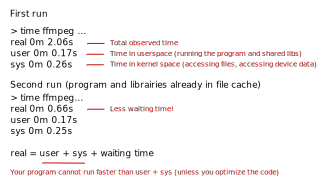
\includegraphics[height=0.7\textheight]{slides/boot-time-toolchain2/using-time-command.pdf}
\end{center}
This gives you the best time that can possibly be achieved (with the fastest storage).
\end{frame}

\setuplabframe {Toolchain optimizations}
{
\begin{itemize}
\item Measure filesystem and \code{ffmpeg} binary size. Time
      the execution of the application.
\item Re-compile the root filesystem using a Thumb2 toolchain
\item Re-compile the root filesystem with the {\em Musl}
      C library instead of {\em uClibc}
\item Find the best toolchain in terms of size and execution time.
\item Have Buildroot generate an external toolchain ({\em SDK})
\end{itemize}
}


\begin{frame}
\frametitle{Lessons from labs: ARM vs Thumb2}
\begin{itemize}
\item Testcase: root filesystem with \code{ffmpeg} and associated
      libraries (from our training labs)
\item Compiled with gcc 9.3, generating {\em ARM} code:\\
      Total filesystem size: 17.6 MB\\
      \code{ffmpeg} size: 227 KB
\item Compiled with gcc 9.3, generating {\em Thumb2} code:\\
      Total filesystem size: 14.3 MB (-18 \%)\\
      \code{ffmpeg} size: 183 KB (-19 \%)
\item Performance aspect: performance apparently slightly improved with Thumb2
      (about 2 \%, but there are slight variations in measured
      execution time, for one run to another).
\end{itemize}
\end{frame}

\begin{frame}
\frametitle{Lessons from labs: musl vs uClibc}
Replacing {\em uClibc} by {\em musl} in our video player lab, keeping
{\em Thumb2}:
\begin{itemize}
   \item Total system size with {\em uClibc}: 14.3 MB
   \item Total system size with {\em Musl}: 14.4 MB
   \item uClibc saves 80 KB (useful), but otherwise no other significant change
    in filesystem and code size. Not a surprise when the system is mostly filled
    with binaries relying on shared libraries.
\end{itemize}
Switching to {\em Musl} as it is supposed to allow for smaller static
binariess, which will be useful in later labs.
\end{frame}
